\subsection{Lựa chọn công nghệ}

Hệ thống bỏ phiếu điện tử được đề xuất trong đồ án được hiện thực hóa theo mô hình kiến trúc phân tầng, trong đó mỗi tầng đảm nhiệm một nhóm chức năng riêng biệt và được xây dựng dựa trên những công nghệ phù hợp nhất với đặc thù nhiệm vụ của tầng đó. Cụ thể, tầng hạ tầng blockchain được triển khai và quản trị thông qua nền tảng \textbf{Chainlaunch}; tầng xử lý nghiệp vụ phía máy chủ (Backend) được xây dựng trên khung kiến trúc \textbf{NestJS}; tầng giao diện trình duyệt (Website Frontend) sử dụng \textbf{React} kết hợp công cụ biên dịch \textbf{Vite} và hệ thống thành phần giao diện \textbf{Material UI}; còn tầng ứng dụng di động (Mobile Frontend) được phát triển trên nền tảng \textbf{Expo} cùng giải pháp thành phần \textbf{React Native Reusables} và \textbf{Tailwind CSS}.

Mục này trình bày tổng quan về các nhóm công nghệ nền tảng nói trên, làm rõ vai trò, đặc điểm kỹ thuật cốt lõi và cơ sở lý luận cho việc lựa chọn từng giải pháp trong bối cảnh của một hệ thống đòi hỏi đồng thời tính bảo mật, hiệu năng và khả năng kiểm chứng cao.

\subsubsection{Chainlaunch -- Nền tảng triển khai và quản trị mạng blockchain}

Chainlaunch là một nền tảng mã nguồn mở (open-source) được thiết kế nhằm đơn giản hóa việc triển khai, vận hành và quản lý các node cũng như toàn bộ mạng lưới blockchain ở cấp độ doanh nghiệp. Mục tiêu cốt lõi của nền tảng này là cho phép nhà phát triển khởi tạo một mạng lưới blockchain phức tạp chỉ trong vòng vài phút, thay vì phải cấu hình thủ công tốn nhiều thời gian và dễ phát sinh sai sót. Trong đồ án, Chainlaunch được sử dụng để dựng và quản trị mạng Hyperledger Fabric làm hạ tầng blockchain cho hệ thống bỏ phiếu. Người dùng có thể tương tác với nền tảng thông qua phương thức linh họat: \textit{Website UI} (giao diện trình duyệt), \textit{CLI} (dòng lệnh), \textit{REST API}, hoặc \textit{Terraform provider} để tự động hóa hạ tầng theo mô hình Infrastructure as Code (IaC).

Về phạm vi hỗ trợ, Chainlaunch cho phép triển khai nhiều nền tảng blockchain phổ biến:

\begin{itemize}
    \item \textbf{Hyperledger Fabric:} Hỗ trợ cấu hình đầy đủ các thành phần như peers, orderers và CAs, với các thuật toán đồng thuận Raft và SmartBFT.

    \item \textbf{Hyperledger Fabric-X:} Một biến thể tối ưu hiệu năng cao (high-throughput) của Fabric, sử dụng cơ chế đồng thuận Arma, tách biệt cấu trúc orderer và committer, đồng thời hỗ trợ dịch vụ truy vấn (query service) dựa trên cơ sở dữ liệu PostgreSQL.

    \item \textbf{Hyperledger Besu:} Hỗ trợ khởi tạo các validators, bootnodes và fullnodes chạy trên thuật toán đồng thuận QBFT.

    \item \textbf{Mở rộng qua plugin:} Cho phép tích hợp thêm các framework blockchain khác nhờ kiến trúc mô-đun có khả năng mở rộng.
\end{itemize}

Về mặt kiến trúc, Chainlaunch được tổ chức thành các khối chức năng (modules) độc lập nhưng phối hợp chặt chẽ. \textit{Deployment Module} xử lý việc cài đặt mạng lưới với khả năng tương thích đa nền tảng cao thông qua các cơ chế quản lý dịch vụ native của hệ điều hành (SystemD trên Linux, LaunchD trên macOS) hoặc môi trường container hóa Docker. \textit{Storage \& Persistence} lưu cấu hình và trạng thái vận hành trong cơ sở dữ liệu nhúng SQLite. Bên cạnh đó còn tích hợp thêm các công nghệ là \textit{Backup Module} (sao lưu chứng chỉ và snapshot qua Restic/S3, AWS EBS hoặc VMware), \textit{Monitoring \& Notifications Module} (giám sát qua ping và metric, cảnh báo qua SMTP, tích hợp sẵn Prometheus, Grafana và block explorer) và \textit{Smart Contract AI (SCAI) Module} (môi trường phát triển chaincode trên trình duyệt có trợ giúp của trí tuệ nhân tạo qua OpenAI hoặc Claude). Kiến trúc tổng thể của nền tảng được minh họa trong Hình~\ref{fig:chainlaunch-arch}.

\begin{figure}[H]
    \centering
    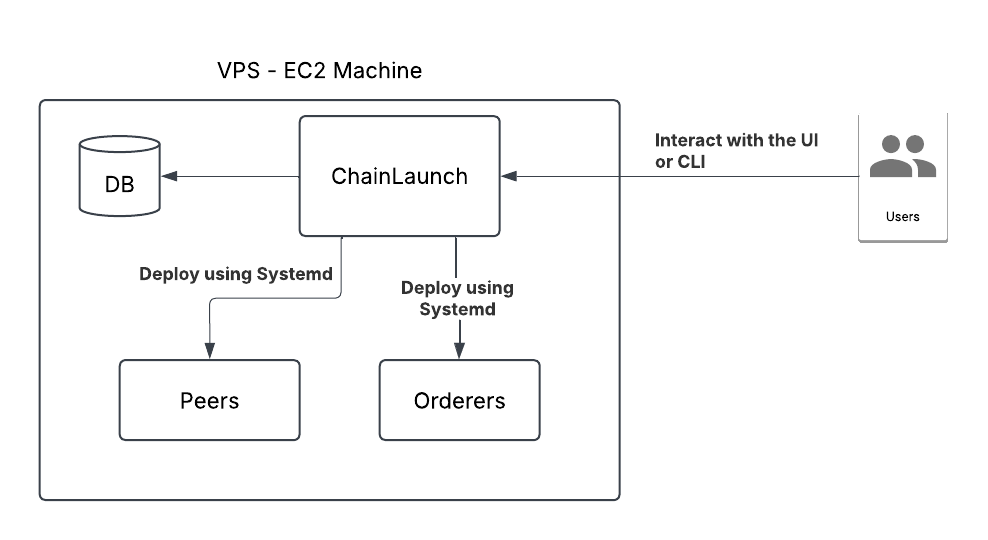
\includegraphics[width=0.95\textwidth, keepaspectratio]{Figures/Chainlaunch-architecture.png}
    \caption{Kiến trúc tổng thể của nền tảng Chainlaunch}
    \label{fig:chainlaunch-arch}
\end{figure}

\subsubsection{Công nghệ tầng Backend}

Tầng Backend đảm nhiệm toàn bộ logic nghiệp vụ, điều phối giao dịch tới mạng blockchain và quản lý dữ liệu ngoài chuỗi. Các công nghệ chủ đạo của tầng này được lựa chọn nhằm cân bằng giữa tính cấu trúc hóa của mã nguồn, độ an toàn kiểu dữ liệu và hiệu năng xử lý.

\begin{itemize}
    \item \textbf{NestJS -- Khung kiến trúc và mô hình quản trị logic:} NestJS chuẩn hóa kiến trúc máy chủ Node.js bằng cách áp dụng nghiêm ngặt mô hình \textit{Dependency Injection} (DI) và \textit{Inversion of Control} (IoC) thông qua cơ chế \textit{Decorators} và \textit{Metadata}. Nhờ đó, logic nghiệp vụ (Services) được phân tách rạch ròi khỏi logic điều phối (Controllers), giúp hệ thống đạt được tính bảo trì và khả năng kiểm thử cao. Việc tích hợp gói \pkg{@nestjs/microservices} còn cho phép trừu tượng hóa các tầng giao thức (TCP, gRPC, Redis Pub/Sub), tạo điều kiện chuyển đổi minh bạch từ mô hình đơn khối (Monolithic) sang phân tán (Microservices).

    \item \textbf{MongoDB và Prisma -- Tầng lưu trữ lai định kiểu:} MongoDB là cơ sở dữ liệu hướng tài liệu (document-oriented) phù hợp với các tập dữ liệu có cấu trúc biến đổi và yêu cầu mở rộng ngang (horizontal scaling); việc sử dụng định dạng \pkg{bson} giúp lưu trữ hiệu quả các cấu trúc phức tạp như cây Merkle. Prisma bổ khuyết nhược điểm thiếu cấu trúc của NoSQL bằng một bản đồ lược đồ (Schema) định nghĩa trước; engine của Prisma được viết bằng ngôn ngữ Rust, cung cấp khả năng tối ưu hóa truy vấn và ngăn chặn các lỗi runtime liên quan đến kiểu dữ liệu -- một yếu tố then chốt khi xử lý dữ liệu nhạy cảm như phiếu bầu.

    \item \textbf{Redis và cơ chế Cache -- Tối ưu hóa hiệu năng:} Hệ thống áp dụng mô hình lưu trữ đa tầng dựa trên công nghệ \pkg{cache-manager} và \pkg{@nestjs/cache-manager}, cho phép đồng bộ hóa trạng thái giữa các instance trong môi trường Microservices, giảm độ trễ mạng và tải trọng lên cơ sở dữ liệu chính. Redis đồng thời đóng vai trò bộ nhớ đệm trung tâm cho tác vụ giới hạn lưu lượng (Rate Limiting) thông qua \pkg{@nestjs/throttler}, giúp bảo vệ tài nguyên hệ thống trước các kịch bản tấn công khai thác hoặc quá tải truy cập nhờ tốc độ xử lý trên bộ nhớ RAM ở ngưỡng ms.
\end{itemize}

\subsubsection{Công nghệ tầng Website Frontend}

Tầng giao diện trình duyệt cung cấp môi trường tương tác cho quản trị viên và cử tri trên trình duyệt. Các công nghệ được lựa chọn nhằm tối ưu đồng thời trải nghiệm phát triển, hiệu năng tải trang và tính nhất quán về thiết kế.

\begin{itemize}
    \item \textbf{React -- Thư viện cốt lõi của tầng giao diện:} React là thư viện JavaScript được sử dụng để xây dựng giao diện người dùng theo mô hình lập trình khai báo (Declarative Programming) và kiến trúc thành phần tái sử dụng. Thông qua cơ chế đối chiếu (Reconciliation) trên DOM ảo (Virtual DOM), React xác định các thay đổi cần thiết và cập nhật chúng lên DOM thật một cách hiệu quả, từ đó giảm số lượng thao tác trực tiếp trên DOM và cải thiện hiệu năng hiển thị. Bên cạnh đó, mô hình luồng dữ liệu một chiều (Unidirectional Data Flow) cùng cơ chế truyền dữ liệu thông qua \pkg{props} giúp tăng tính minh bạch, khả năng dự đoán và khả năng bảo trì của ứng dụng.


    \item \textbf{Vite -- Công cụ xây dựng và tối ưu hóa chu kỳ phát triển:} Trong giai đoạn phát triển, Vite tận dụng tính năng ES Modules nguyên bản của trình duyệt cùng bộ biên dịch \textit{esbuild} (viết bằng ngôn ngữ Go) để loại bỏ giai đoạn đóng gói toàn bộ mã nguồn, nhờ đó giảm thời gian khởi động môi trường (Cold Start) xuống mức mili-giây. Trong giai đoạn biên dịch sản phẩm, Vite sử dụng \textit{Rollup} để thực thi các kỹ thuật phân tách mã động (Code-Splitting), loại bỏ mã thừa (Tree-Shaking) và tối ưu chiến lược tải trước tài nguyên, qua đó giữ kích thước tệp đầu ra ở mức tối thiểu và cải thiện trực tiếp các chỉ số Core Web Vitals.

    \item \textbf{Material UI và Emotion -- Hệ thống thiết kế và giải pháp CSS-in-JS:} Material UI (MUI) là thư viện giao diện người dùng cung cấp tập hợp các thành phần được xây dựng dựa trên ngôn ngữ thiết kế Material Design của Google. Kết hợp với giải pháp CSS-in-JS của Emotion (\pkg{@emotion/react} và \pkg{@emotion/styled}), MUI cho phép định nghĩa và quản lý phong cách trực tiếp trong thành phần giao diện, hạn chế xung đột giữa các lớp CSS và hỗ trợ tùy biến giao diện động trong quá trình thực thi. Bên cạnh đó, cơ chế quản lý giao diện tập trung giúp duy trì tính nhất quán về màu sắc, kiểu chữ và khoảng cách hiển thị trên toàn bộ hệ thống.

\end{itemize}

\subsubsection{Công nghệ tầng Mobile Frontend}

Tầng ứng dụng di động cho phép cử tri thực hiện bỏ phiếu trực tiếp trên thiết bị cá nhân. Để bảo đảm khả năng phát triển đa nền tảng từ một kho mã nguồn duy nhất cùng giao diện linh hoạt, tầng này được xây dựng dựa trên hai trụ cột công nghệ chính.

\begin{itemize}
    \item \textbf{Expo -- Nền tảng thực thi và quản lý vòng đời ứng dụng đa nền tảng:} Expo cung cấp giải pháp toàn diện để phát triển, biên dịch và vận hành ứng dụng trên iOS, Android và Web từ một kho mã nguồn duy nhất. Nền tảng này cung cấp các API đồng bộ giúp mã JavaScript tương tác trực tiếp với tính năng native của thiết bị (lưu trữ an toàn, định vị, camera) mà không cần can thiệp vào mã nguồn Java/Kotlin hay Objective-C/Swift. Cơ chế \textit{Expo Router} áp dụng mô hình định tuyến dựa trên tệp tin (File-based Routing), tự động hóa luồng điều hướng và tối ưu việc phân tách tài nguyên cũng như quản lý vòng đời của các màn hình.

    \item \textbf{React Native Reusables và Tailwind CSS -- Thư viện xây dựng UI:} Sự kết hợp này lấy cảm hứng trực tiếp từ mô hình \textit{Shadcn UI} trên nền tảng web, phân tách rạch ròi giữa logic vận hành và lớp trình bày của ứng dụng. Thay vì cung cấp các cấu phần đóng gói cứng nhắc, React Native Reusables (RNR) đưa cho nhà phát triển những component đơn giản (dựa trên \pkg{@rn-primitives}) đã được lập trình sẵn toàn bộ logic phức tạp bên dưới; nhà phát triển chỉ cần sao chép và tùy biến mã nguồn trực tiếp trong dự án, qua đó nắm quyền kiểm soát tuyệt đối và tránh phụ thuộc vào mã nguồn ẩn của bên thứ ba. Để hoàn thiện lớp vỏ ngoài, hệ thống sử dụng Tailwind CSS làm ngôn ngữ định kiểu theo hướng tiện ích (Utility-First): nhà phát triển chỉ cần gắn các \pkg{className} ngắn gọn để chỉ định màu sắc, khoảng cách và bố cục.
\end{itemize}
